\section{灵敏度与鲁棒性分析}\label{sec:sens}

上一章说明了模型选择对结论的影响，本章考察在模型选定之后参数取值的影响。做法是一次只改一个量、其余全部不变，共十三个扰动算例，全部沿用问题三的求解器、网格、时间步安排与判据，基准为 $t_{\rm dry}=57.5316$~h。这样安排的目的不是穷举组合，而是分辨哪些量的不确定性会真正传到结论上：题给参数中有的是实测值、有的是经验公式的拟合系数，可靠程度并不相同，需要知道各自的权重。

\subsection{参数扰动的效应与弹性}

对每个参数取 $\pm10\%$ 的双侧扰动，这种一次一变的设计便于把效应直接归属到单个参数，也是干燥过程参数不确定性分析的常用做法\upcite{ferrari2016param}。效应用无量纲弹性度量

\begin{equation}
E=\frac{\Delta t_{\rm dry}/t_{\rm dry}}{\Delta p/p},
\label{eq:elastic}
\end{equation}

式~\eqref{eq:elastic} 的含义是参数变化 $1\%$ 时停时随之变化的百分数，符号表示方向。五个物理量的结果列于表~\ref{tab:sens}。

\begin{table}[H]
\centering
\caption{参数 $\pm10\%$ 扰动对烘干时长的影响（基准 57.5316~h）}\label{tab:sens}
\begin{tabular}{lccccc}
\toprule
\multirow{2}{*}{扰动量} & \multicolumn{2}{c}{上调 $10\%$} & \multicolumn{2}{c}{下调 $10\%$} & \multirow{2}{*}{弹性区间} \\
\cmidrule(lr){2-3}\cmidrule(lr){4-5}
 & $t_{\rm dry}$/h & 相对变化 & $t_{\rm dry}$/h & 相对变化 & \\
\midrule
扩散系数 $D$        & 52.9223 & $-8.01\%$  & 63.1919 & $+9.84\%$  & $-0.80\ \text{至}\ -0.98$ \\
判据阈值 $C_{\rm th}$ & 46.0142 & $-20.02\%$ & 76.1486 & $+32.36\%$ & $-2.00\ \text{至}\ -3.24$ \\
传质系数 $h_m$      & 56.9545 & $-1.00\%$  & 58.2672 & $+1.28\%$  & $-0.10\ \text{至}\ -0.13$ \\
空气水分浓度 $C_a$   & 57.6522 & $+0.21\%$  & 57.4299 & $-0.18\%$  & $+0.02$ \\
传热系数 $h$        & 57.5245 & $-0.01\%$  & 57.5404 & $+0.02\%$  & $\approx 0$ \\
\bottomrule
\end{tabular}
\end{table}

五行的效应量级相差三个数量级，说明各参数的地位完全不对等。扩散系数的弹性接近 $-1$，即它的相对误差几乎一比一地传到停时上；传质系数的弹性只有它的八分之一；空气水分浓度几乎无影响，因为它比药材含水率小两个数量级，$\pm10\%$ 的变动对表面浓差的改变微乎其微；传热系数的效应更是低到 $0.01\%$ 的量级。图~\ref{fig:sensitivity} 按效应绝对值把全部扰动排序。

\begin{figure}[htbp]
  \centering
  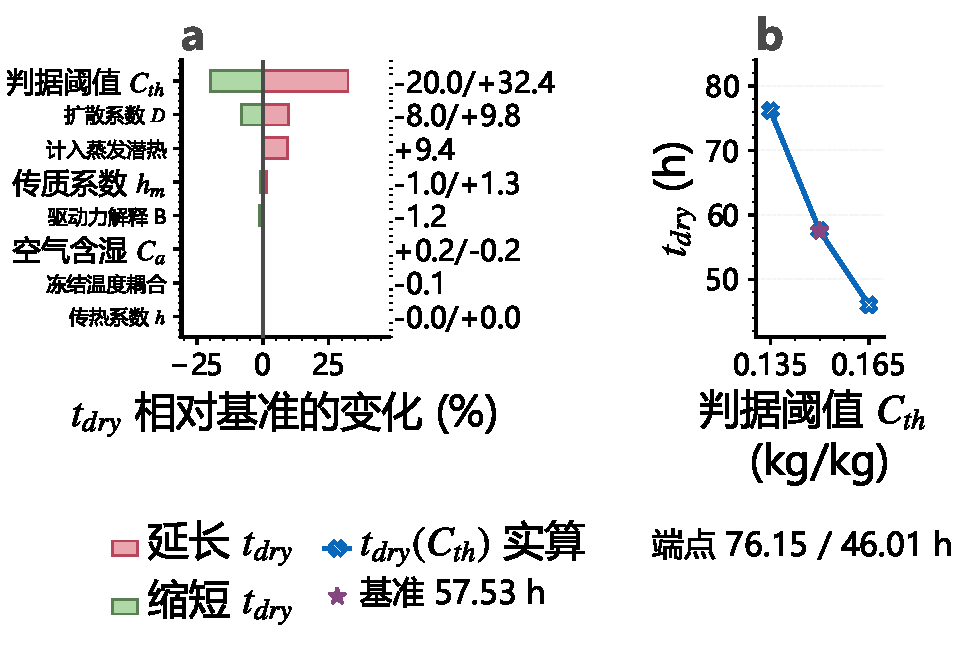
\includegraphics[width=0.9\textwidth,height=0.8\textheight,keepaspectratio]{../figures/fig_sensitivity.pdf}
  \caption{问题 3 的灵敏度与鲁棒性。a：龙卷风图，13 个扰动算例按物理量合并为
  8 行并按效应绝对值排序，右侧为延长、左侧为缩短，右侧刻度给出两侧的相对变化
  百分数；扩散系数与判据阈值的效应量级明显领先，传热系数则几乎无影响，这与预热
  远快于干燥的时间尺度分离一致。b：判据阈值的单侧扰动效应明显不对称，下调阈值
  造成的延长幅度大于上调阈值造成的缩短幅度，故阈值的取法需在正文中明确声明。}
  \label{fig:sensitivity}
\end{figure}

左图的横条长度自上而下急剧衰减，最长的两条属于判据阈值与扩散系数，最短的一条几乎缩成一根竖线，这与表~\ref{tab:sens} 的排序一致。传热系数那一行的近乎消失有明确的物理解释：温度场在两小时内就已进入准稳态，其后表面换热强弱不再改变任何事情，限制环节完全在内部水分扩散一侧。右图把阈值的两侧效应单独并置，可以看到两根条并不等长，下调一侧明显更长。

\subsection{判据阈值的主导地位与不对称性}

效应最大的量不是物理参数而是判据阈值本身：阈值从 $0.15$ 上调到 $0.165$~kg/kg 使停时缩短 $20.02\%$，下调到 $0.135$~kg/kg 使停时延长 $32.36\%$，后者是前者的 $1.6164$ 倍。这个不对称性来自扩散系数随变干而减小：越接近干透，含水率下降越慢，因此在低含水率一侧多要求一点点，就要付出很多时间。它给出的工程含义是明确的——若把合格标准从 $0.15$ 收紧一成，烘干时间要增加三成以上，收紧标准的代价远大于放宽标准的收益。

这也说明前文为何反复强调阈值的取法。阈值不是待估参数而是题目给定的外部标准，本文全程严格取 $0.15$~kg/kg 并按“各处”解释为径向最大值；此处的扰动只用于说明该标准的敏感程度，不构成对基准结果的修正。相应地，两个阈值扰动算例的停时（$46.0142$ 与 $76.1486$~h）落在题面所给的两到三天之外，这是因为它们改动的是判据本身而不是模型，不能据此判定模型失效。

\subsection{三项建模选择的影响}

除参数之外，本文在建模阶段还作过三项选择，它们无法用 $\pm10\%$ 扰动衡量，只能整支重算，结果列于表~\ref{tab:sens-model}。

\begin{table}[H]
\centering
\caption{三项建模选择的整支对照（基准 57.5316~h）}\label{tab:sens-model}
\begin{tabular}{lcc}
\toprule
对照处理 & $t_{\rm dry}$/h & 相对基准 \\
\midrule
表面通量改按体积浓度作差（假设（4）的另一解释） & 56.8367 & $-1.21\%$ \\
温度场整段冻结为空气温度（切断温度对传质的耦合） & 57.4462 & $-0.15\%$ \\
热方程计入蒸发潜热汇项（假设（3）的对照） & 62.9380 & $+9.40\%$ \\
\bottomrule
\end{tabular}
\end{table}

第一项针对表面传质驱动力的写法。本文按假设（4）取药材侧与空气侧含水率的直接差值；另一种解释把两侧都换成体积浓度作差，等价于把空气侧参考浓度取为零。改按后者，停时变为 $56.8367$~h，只差 $1.21\%$，但达标时的表面含水率由 $0.0526$ 降到 $0.0026$~kg/kg——驱动力被抬高后表面被过度抽干，而这一变化对轴线的达标时刻影响甚微。参考基的模糊性因此不影响结论的量级，其效应比阈值敏感度小一个半数量级。

第二项是一个诊断算例：把温度场固定为空气温度、只解水分方程，停时只变化 $0.15\%$。这证实了前面从时间尺度分离得出的判断——温度场在恒温平台段确实可以视为传质的一个参数而非独立变量。需要注意这个结论只在整体停时的层面成立，预热段的温度仍在爬升、扩散系数随之变化，那一段不能冻结，问题一给出的正是这一段的分布。

第三项影响最大也最需要如实说明。题目给出的四个物性附录中都没有蒸发潜热，附录 3 的比热容公式也未提供潜热项，因此本文的热方程按假设（3）不含潜热汇。为界定这一选择的影响，另设一支在热方程中加入潜热汇，潜热取 $2.4\times10^6$~J/kg——这是水在该温区的量级参考值，并非题给参数，只用于对照而不进入任何交付结果。该支的停时为 $62.9380$~h，比基准慢 $9.40\%$。这是三项选择中量级最大的一项，本文的态度是登记而不宣称可忽略：若题目提供潜热数据，停时应向偏慢一侧修正约一成。

\subsection{结论的鲁棒性区间}

% 本段中文里连排多段行内数学，断行点稀疏，给最后一遍断行额外的伸展余量以免溢出版心。
{\emergencystretch=2.5em
把改动判据本身的两个算例排除在外，其余十一个算例的停时落在 $52.9223$ 至 $63.1919$~h 之间，折合 $2.20$ 至 $2.63$ 天，全部仍在题面所给的两到三天之内。也就是说，即使把最敏感的物理参数拉偏一成、或者改变潜热与驱动力的处理方式，结论的定性与工程量级都不变。连同基准在内的十四支算例，守恒残差最大为 $5.737\times10^{-13}$，与基准同处机器精度，说明扰动没有把任何一支算例推离数值可靠的区间。\par}

按敏感度排序还给出一条明确的改进方向：若要提高预测精度，应优先获取更可靠的扩散系数与潜热数据，而不是细化表面传热系数的测量——后者的效应比前者小三个数量级。
